\documentclass[12pt,a4paper]{article}
\usepackage{amsmath}
\usepackage{fontspec}
\IfFontExistsTF{Times New Roman}{\setmainfont{Times New Roman}}{\setmainfont{Liberation Serif}}
\setsansfont{Liberation Sans}
\setmonofont{Liberation Mono}[Scale=0.88]
\usepackage{tikz}
\usetikzlibrary{arrows.meta,positioning,shapes.geometric,fit,calc}
\usepackage[edges]{forest}
\usepackage[margin=2cm]{geometry}
\usepackage{graphicx,booktabs,array,multirow,float,caption,enumitem,xcolor}
\usepackage[hidelinks]{hyperref}
\usepackage{titlesec}
\titleformat{\section}{\large\bfseries}{\thesection.}{0.5em}{}
\titleformat{\subsection}{\normalsize\bfseries}{\thesubsection.}{0.5em}{}
\setlist{nosep,leftmargin=1.4em}
\linespread{1.08}
\captionsetup{font=small,labelfont=bf}
\graphicspath{{figures/}{../outputs/figures/}}
\newcommand{\code}[1]{\texttt{#1}}
\setlength{\parskip}{3pt}
\renewcommand{\figurename}{Hình}
\renewcommand{\tablename}{Bảng}

\begin{document}

\begin{center}
{\small ĐẠI HỌC QUỐC GIA HÀ NỘI -- TRƯỜNG ĐẠI HỌC CÔNG NGHỆ}\\[4pt]
{\Large\bfseries BÁO CÁO BÀI THI GIỮA KỲ}\\[2pt]
{\large Môn Phân tích và khai phá dữ liệu}\\[6pt]
{\bfseries Phân cụm khách hàng sàn thương mại điện tử}\\[6pt]
Phạm Thanh Trung -- MSSV 24022476
\end{center}

\noindent\textbf{Tham số theo MSSV} ($s = 24022476$): $a = s \bmod 5 = 1$, $b = (s \operatorname{div} 10) \bmod 5 = 2$, $c = (s \operatorname{div} 100) \bmod 5 = 4$, suy ra $N = 220$ bản ghi, $\ge 10$ thuộc tính đầu vào, $\ge 13$ bản ghi ngoại lai.

\noindent\textbf{Quy trình:} CRISP-DM (Hình~\ref{fig:pipeline}). Mã nguồn gồm 5 notebook chạy tuần tự (\code{notebooks/01}--\code{05}), seed cố định 2476; toàn bộ pipeline đã được chạy lại từ đầu, không lỗi và cho dữ liệu giống hệt từng byte. \textbf{Nguyên tắc chống rò rỉ:} dữ liệu sạch, nhật ký can thiệp và nhãn \code{true\_segment} chỉ được dùng để \emph{đối chiếu} (mục cuối mỗi câu) và đánh giá ở câu e; không dùng để điền giá trị, chọn thuộc tính, scaler, PCA hay số cụm.

\noindent\textbf{Mục tiêu và tiêu chí thành công} (đặt trước khi có kết quả): các cụm diễn giải được bằng ngôn ngữ nghiệp vụ; 3--6 cụm; mỗi cụm $\ge 5\%$; ARI so với phân khúc ẩn $\ge 0{,}6$; silhouette $\ge 0{,}25$.


\begin{figure}[H]\centering
\begin{tikzpicture}[font=\footnotesize,
  stage/.style={draw,rounded corners=3pt,fill=blue!8,align=center,minimum height=1.95cm,text width=2.35cm,font=\scriptsize},
  data/.style={draw,shape=cylinder,shape border rotate=90,aspect=0.18,fill=orange!12,align=center,minimum height=0.95cm,text width=2.35cm,font=\scriptsize},
  ref/.style={draw,dashed,rounded corners=2pt,fill=gray!8,align=center,text width=5.6cm,font=\scriptsize},
  arr/.style={-{Stealth[length=2mm]},thick}, darr/.style={-{Stealth[length=2mm]},dashed,gray}, node distance=0.42cm]
\node[stage] (a) {\textbf{a.} Sinh dữ liệu\\4 phân khúc ẩn\\nhiễu, ngoại lai, thiếu};
\node[stage,right=of a] (b) {\textbf{b.} Data\\Understanding\\thống kê, tương quan, LOF};
\node[stage,right=of b] (c) {\textbf{c.} Preprocessing\\NaN ô bất khả\\KNN ($k=20$)};
\node[stage,right=of c] (d) {\textbf{d.} Preparation\\log1p, bỏ dư thừa\\StandardScaler, PCA};
\node[stage,right=of d] (e) {\textbf{e.} K-Means\\so sánh trước/sau\\ARI, NMI, hồ sơ cụm};
\node[data,below=0.7cm of a] (da) {customers\_dirty\\(220 × 13)};
\node[data,below=0.7cm of b] (db) {b\_outlier\_\\candidates};
\node[data,below=0.7cm of c] (dc) {customers\_\\preprocessed};
\node[data,below=0.7cm of d] (dd) {customers\_prepared\\(220 × 5 PC)};
\node[data,below=0.7cm of e] (de) {cluster\_\\assignments};
\foreach \x in {a,b,c,d,e} \draw[arr] (\x) -- (d\x);
\draw[arr] (da) -- (b); \draw[arr] (db) -- (c); \draw[arr] (dc) -- (d); \draw[arr] (dd) -- (e);
\draw[arr] (a.north) |- ++(0,0.4) -| node[pos=0.25,above,font=\scriptsize]{dữ liệu bẩn, biến đổi tối thiểu (kịch bản ``trước xử lý'')} (e.north);
\node[ref,below=0.8cm of dc] (cl) {customers\_clean, injection\_log, true\_segment\\\textbf{chỉ dùng để đối chiếu}};
\draw[darr] (cl.west) -| (db.south); \draw[darr] (cl.east) -| ([xshift=6mm]de.south);
\draw[darr] (cl) -- (dc);
\end{tikzpicture}
\caption{Pipeline của dự án. Mũi tên liền: luồng dữ liệu; mũi tên đứt: dữ liệu sạch và nhãn chỉ dùng ở các mục đối chiếu (b, c) và đánh giá (e). Đường phía trên: dữ liệu bẩn đi thẳng vào câu e làm kịch bản ``trước xử lý''.}\label{fig:pipeline}
\end{figure}

%=====================================================================
\section{Câu a. Thiết kế và sinh dữ liệu}

\subsection{Thuộc tính}
Khung thiết kế: RFM (Recency, Frequency, Monetary) kết hợp nhân khẩu học và hành vi tương tác. 13 thuộc tính đầu vào, phân loại theo giáo trình \emph{Data understanding}:

\begin{table}[H]\centering\footnotesize
\begin{tabular}{@{}p{3.6cm}p{2.5cm}p{4.9cm}p{5.6cm}@{}}\toprule
Thuộc tính & Kiểu & Phân phối sinh & Ý nghĩa, lý do chọn\\\midrule
age & số rời rạc & Normal chặn [18, 70] & Tuổi; khả năng chi tiêu\\
gender & nhị phân đối xứng & Bernoulli(0,5), độc lập & \emph{Phép thử}: thuộc tính không mang cấu trúc cụm\\
region & nominal & Categorical, độc lập & Logistics, khuyến mãi theo vùng\\
membership\_tier & ordinal & Rời rạc hóa orders$\times$AOV & Hạng thành viên\\
tenure\_months & số rời rạc & Gamma, $\le (\text{age}-16)\cdot 12$ & Độ gắn bó\\
annual\_income & số liên tục & Log-normal & Khả năng chi trả; lệch phải\\
orders\_per\_year & số rời rạc & Negative Binomial & F; biến đếm quá phân tán\\
avg\_order\_value & số liên tục & Log-normal, tương quan log với income & M\\
days\_since\_last\_purchase & số rời rạc & Exp$(365/\text{orders})$ + nhiễu riêng & R; nhận diện khách sắp rời bỏ\\
return\_rate & tỷ lệ [0,1] & Beta & Chi phí vận hành\\
discount\_usage\_rate & tỷ lệ [0,1] & Beta & Độ nhạy khuyến mãi\\
sessions\_per\_month & số rời rạc & NB, mean $= 3 + 0{,}7\cdot$orders & Tương tác; dư thừa có chủ đích\\
preferred\_category & nominal & Categorical theo phân khúc & Gợi ý sản phẩm\\\bottomrule
\end{tabular}
\end{table}

\subsection{Cơ chế sinh và giả định}
Dữ liệu sinh theo 4 \textbf{phân khúc ẩn} (VIP 30, Săn khuyến mãi 70, Trung thành 60, Mới/ít hoạt động 60), mỗi phân khúc có bộ tham số riêng. Tỷ lệ lệch có chủ đích để gần thực tế. Lý do chọn phân phối: thu nhập và giá trị đơn luôn dương và lệch phải (mean $>$ median) nên dùng log-normal; số đơn là biến đếm quá phân tán nên dùng Negative Binomial thay vì Poisson; tỷ lệ bị chặn trong $[0,1]$ nên dùng Beta. Recency được suy ra từ tần suất mua (thời gian chờ của quá trình Poisson), nhân nhiễu log-normal và cộng thành phần ``ngừng mua'' để không dư thừa hoàn toàn với số đơn.

\textbf{Hạn chế:} tham số do người thiết kế chọn; giả định IID, không có yếu tố mùa vụ; các phân khúc có thể tách biệt hơn thực tế nên kết quả phân cụm lạc quan; N nhỏ.

\subsection{Làm bẩn dữ liệu}
Thứ tự: \textbf{nhiễu $\to$ ngoại lai $\to$ giá trị thiếu} (để nhiễu không làm lệch ngoại lai đã thiết kế và ô thiếu không xóa mất ngoại lai). Mọi thay đổi ghi vào \code{injection\_log.csv}.
\begin{itemize}
\item \textbf{Nhiễu (3 cột):} AOV $\times(1+\mathcal N(0;0{,}08))$, income $\times(1+\mathcal N(0;0{,}05))$ (nhiễu nhân cho biến log-normal); sessions $+\mathcal N(0;2)$ (nhiễu cộng cho biến đếm).
\item \textbf{Ngoại lai (15 bản ghi, sửa trên dòng có sẵn để giữ N = 220):} 5 lỗi đơn biến (tuổi 150 và 3, AOV $-450$, return\_rate 2,5, sessions 900); 3 lỗi logic đa biến (18 tuổi nhưng gắn bó 96 tháng; 80 đơn/năm nhưng 180 ngày chưa mua; hạng Platinum nhưng chi tiêu rất thấp); 7 ngoại lai \emph{hợp lệ} (4 khách sỉ, 3 siêu VIP).
\item \textbf{Giá trị thiếu (3 cột):} age MCAR 5\% (11 ô), annual\_income \textbf{MAR} theo tenure 10\% (22 ô), preferred\_category MCAR 4\% (9 ô).
\end{itemize}
Lưu \code{customers\_clean.csv}, \code{customers\_dirty.csv}, \code{injection\_log.csv}; các đặc điểm cài sẵn được ghi trước vào \code{expected\_findings.md} để kiểm chứng câu b.

%=====================================================================
\section{Câu b. Data Understanding}
Phân tích chỉ trên dữ liệu bẩn. Rủi ro thiên kiến (người sinh dữ liệu cũng là người phân tích) được giảm bằng cách ghi giả thuyết trước khi chạy và ghi nhận cả các phát hiện sai.

\begin{figure}[H]\centering
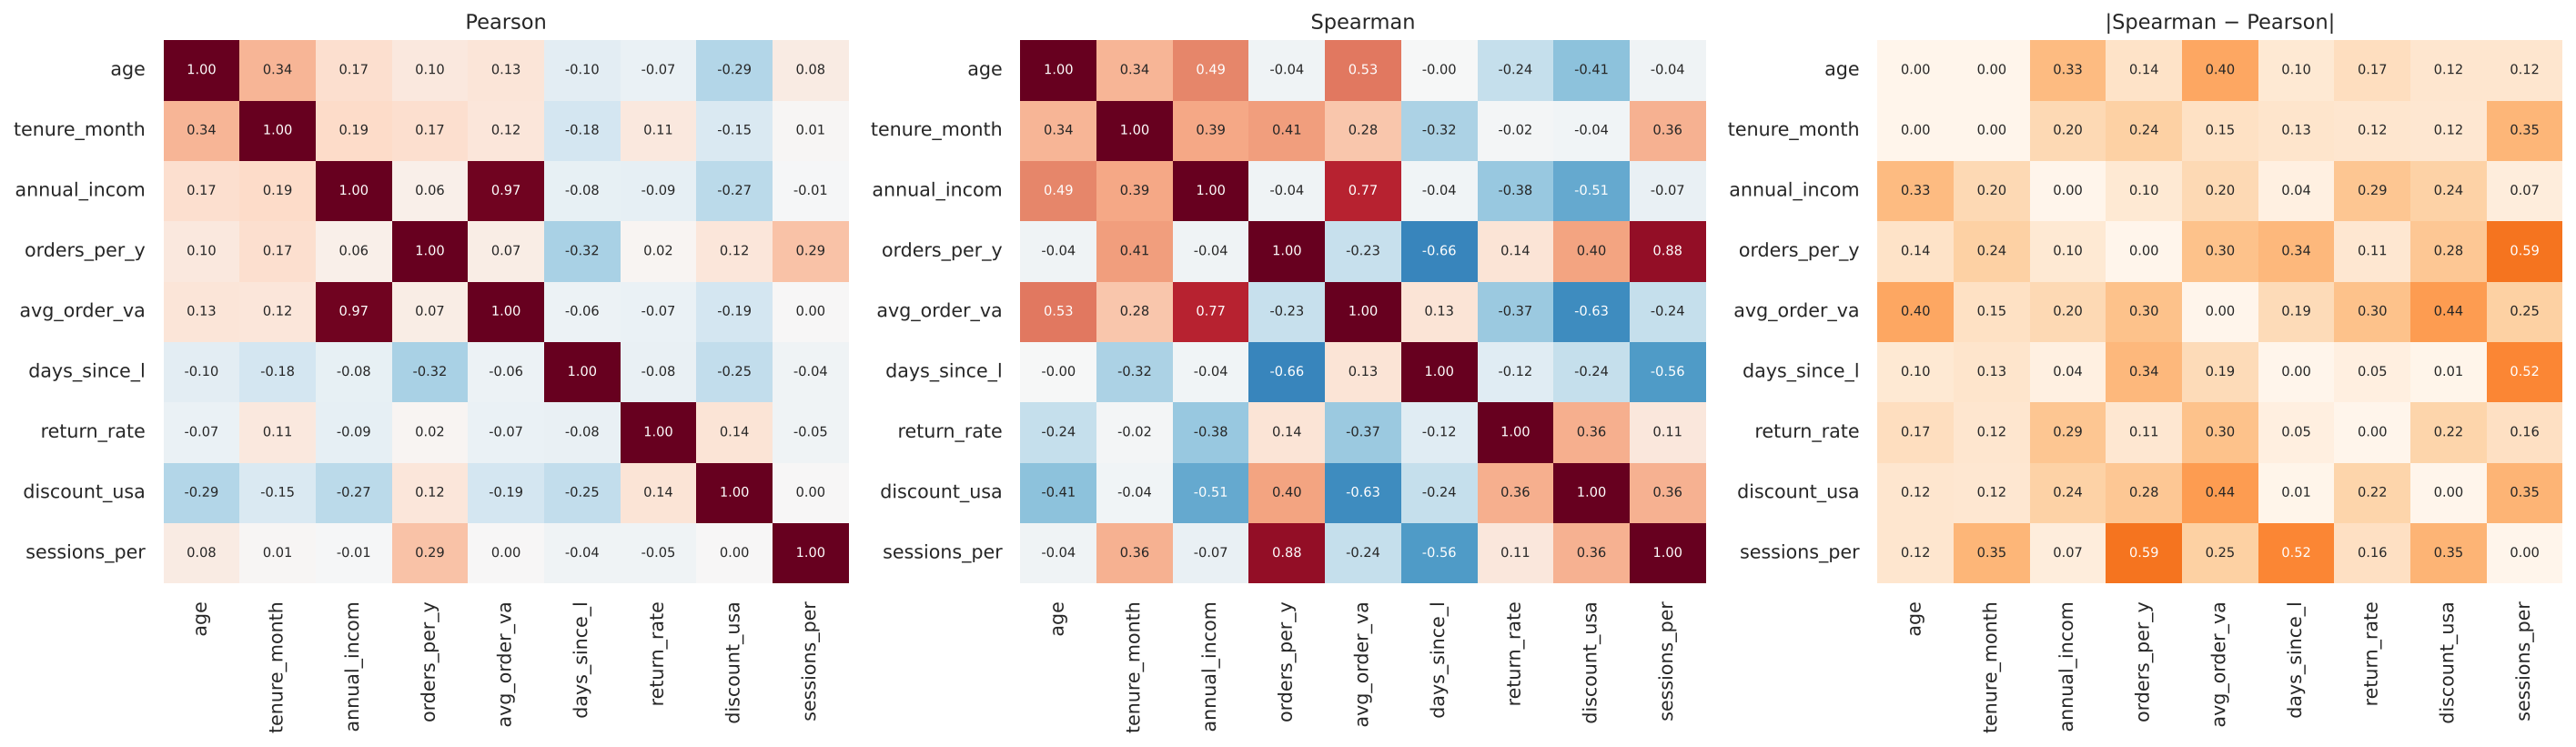
\includegraphics[width=\linewidth]{b_corr_heatmaps.png}
\caption{Pearson, Spearman và $|$Spearman $-$ Pearson$|$ trên dữ liệu bẩn.}\label{fig:corr}
\end{figure}

\textbf{Các phát hiện chính}
\begin{enumerate}
\item \textbf{Lệch phải mạnh, mean không đại diện:} mean/median của AOV 2,66, của recency 3,88; skewness AOV 8,0, sessions 12,0. Midrange AOV gấp 44 lần median. log1p đưa skewness của orders, sessions, recency về gần 0.
\item \textbf{Pearson bị ngoại lai bóp méo theo cả hai hướng} (Hình~\ref{fig:corr}): orders--sessions Pearson 0,29 nhưng Spearman 0,88 (một ô sessions = 900); income--AOV Pearson 0,97 nhưng Spearman 0,77 (điểm đòn bẩy của siêu VIP).
\item \textbf{Thuộc tính dư thừa:} orders--sessions (Spearman 0,88), tier--tổng chi tiêu (0,885).
\item \textbf{Thiếu có dấu hiệu MAR:} nhóm thiếu income có tenure thấp hơn (median 7 so với 24 tháng, Mann--Whitney $p = 0{,}0018$), nhưng \textbf{sau hiệu chỉnh Holm} cho 36 kiểm định $p = 0{,}064$: có dấu hiệu nhưng chưa đủ bằng chứng.
\item \textbf{gender, region không liên hệ} với thuộc tính nào ($\chi^2$, mọi $p > 0{,}24$).
\item \textbf{IQR thang gốc gắn cờ 29\% dữ liệu} (64/220), chủ yếu do lệch; trên thang log còn 21 dòng. z-score bị hiệu ứng che khuất (ô 900 làm std sessions tăng từ 23 lên 64).
\end{enumerate}

\textbf{Phát hiện ngoại lai.} Năm phương pháp: ràng buộc (cứng và mềm), IQR thang gốc, IQR thang log, z-score, LOF. Kết quả phân loại (chỉ từ dữ liệu bẩn): 6 \emph{bất khả}, 3 \emph{đáng ngờ}, 17 \emph{cực trị hợp lý}.

\begin{table}[H]\centering\small
\begin{tabular}{@{}lrrrccc@{}}\toprule
Phương pháp & Gắn cờ & Precision & Recall & Lỗi đơn biến & Lỗi logic & Hợp lệ\\\midrule
Ràng buộc cứng & 6 & 1,00 & 0,40 & 5/5 & 1/3 & 0/7\\
IQR 1,5 thang gốc & 64 & 0,22 & 0,93 & 5/5 & 2/3 & 7/7\\
IQR 1,5 thang log & 21 & 0,52 & 0,73 & 4/5 & 0/3 & 7/7\\
LOF ($k = 20$) & 7 & 1,00 & 0,47 & 0/5 & 0/3 & 7/7\\
\textbf{Phân loại tổng hợp} & 26 & 0,58 & \textbf{1,00} & 5/5 & 3/3 & 7/7\\\bottomrule
\end{tabular}
\caption{Đối chiếu với nhật ký can thiệp. Không xếp nhầm khách thật nào vào nhóm ``bất khả''.}
\end{table}

\textbf{Những chỗ phân tích sai hoặc phát hiện lỗi thiết kế:} (i) giả thuyết ``LOF bắt được lỗi logic'' sai (0/3); lỗi logic chỉ phát hiện được bằng tri thức nghiệp vụ. (ii) Ràng buộc mềm ``$\ge 50$ đơn nhưng $\ge 120$ ngày chưa mua'' gắn cờ nhầm một khách thật đang rời bỏ (C0091), lộ ra \textbf{lỗi thiết kế ở câu a}: lỗi logic C0205 không phân biệt được với hành vi tự nhiên; vì vậy được hạ xuống ``đáng ngờ''. (iii) Kết luận MAR không đạt ý nghĩa sau hiệu chỉnh: sai lầm loại II do chỉ có 22 ô thiếu.

\textbf{Ảnh hưởng dự kiến đến phân cụm:} chênh lệch thang đo khiến khoảng cách Euclid bị AOV chi phối; cực trị kéo centroid và có thể tạo cụm 1--3 điểm; thuộc tính dư thừa nhân đôi trọng số; giá trị thiếu cần điền vì K-Means không chạy với NaN; thuộc tính không mang cấu trúc làm loãng khoảng cách.

%=====================================================================
\section{Câu c. Data Preprocessing}
Giữ nguyên thang đo gốc (để mô tả cụm bằng đơn vị nghiệp vụ); không khôi phục từ dữ liệu sạch.

\begin{table}[H]\centering\small
\begin{tabular}{@{}p{2.8cm}p{5.4cm}p{7.6cm}@{}}\toprule
Vấn đề & Xử lý & Cơ sở\\\midrule
6 ô bất khả & Đặt riêng ô sai về NaN, điền lại, gắn cờ \code{invalid\_cols} & Giá trị sai không chứa thông tin; chỉ gắn cờ thì giá trị sai vẫn vào khoảng cách; kẹp biên là bịa giá trị; xóa dòng mất 12 ô đúng. C0211: đặt tenure về NaN (tuổi 18 hợp lệ)\\
3 dòng đáng ngờ, 17 cực trị hợp lý & Giữ nguyên, gắn cờ \code{outlier\_type} & Không mặc định loại bỏ; là khách giá trị cao thật; giảm ảnh hưởng ở câu d\\
48 ô thiếu & KNN, $k = 20$, trọng số khoảng cách & Thí nghiệm che rồi điền lại (dưới)\\
Nhiễu & Không làm trơn & Thí nghiệm binning (dưới)\\\bottomrule
\end{tabular}
\end{table}

\textbf{Chọn phương pháp điền mà không dùng dữ liệu sạch.} Lặp 20 lần: che ngẫu nhiên 10\% giá trị đang có, điền bằng 19 cấu hình (median/mode, median theo nhóm tenure, theo hạng, KNN với $k \in \{1,\dots,30\}$, hai kiểu trọng số), đo MAE/IQR. KNN với $k \ge 7$ tốt hơn median khoảng 30\%; $k = 1$ tệ gần bằng median; mặc định $k = 5$ không tối ưu. Đường sai số phẳng từ $k = 10$ đến 30; chọn $k = 20$ theo quy tắc một sai số chuẩn.

\begin{figure}[H]\centering
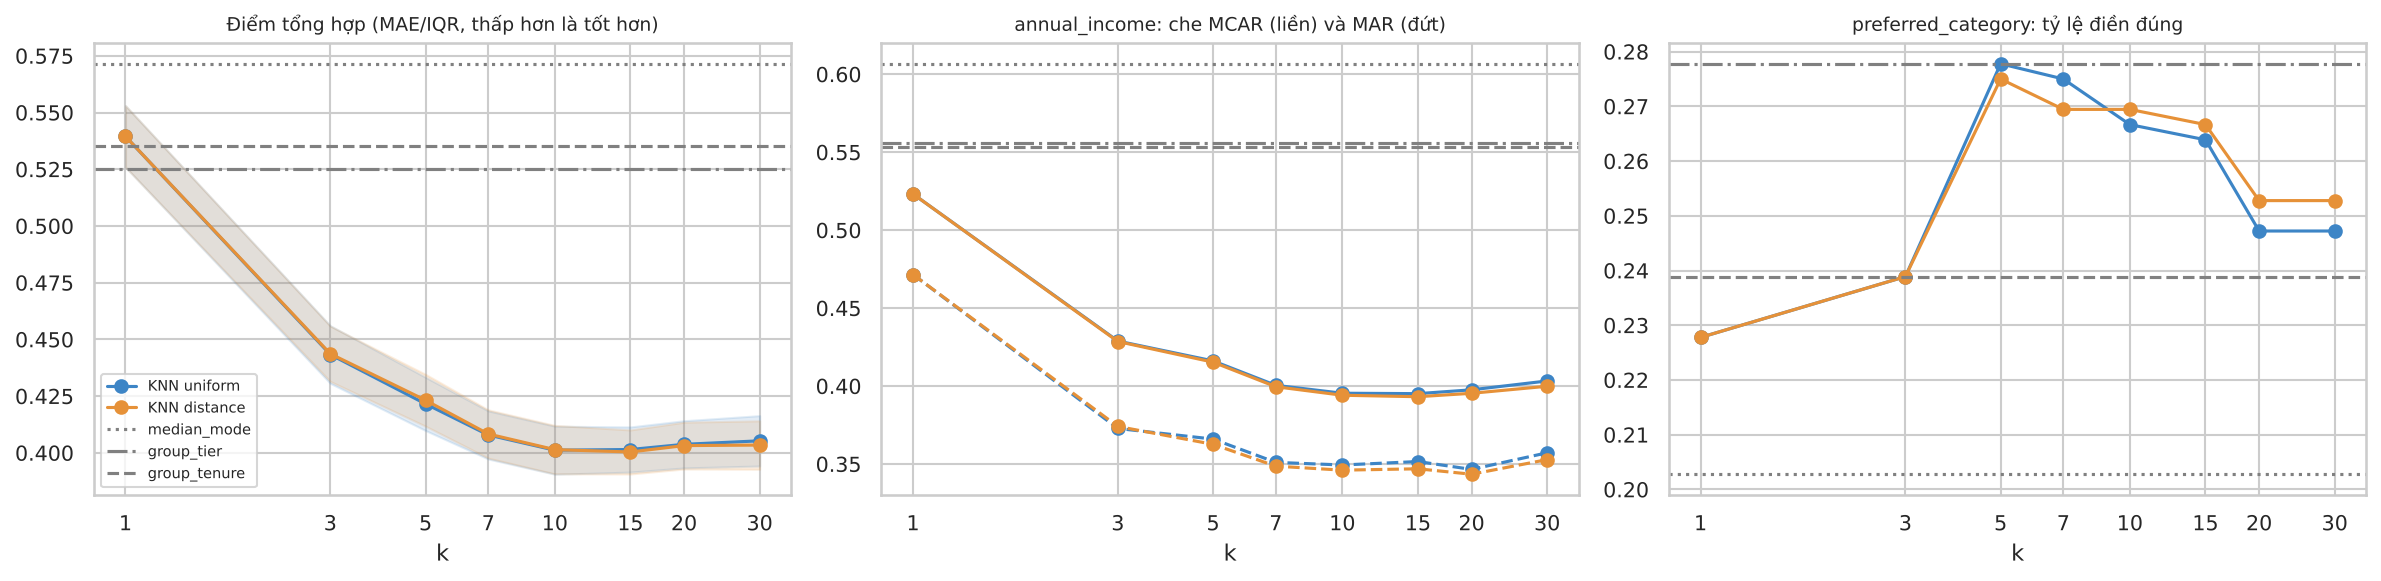
\includegraphics[width=\linewidth]{c_mask_experiment.png}
\caption{Thí nghiệm che rồi điền lại: sai số theo $k$ và so với các phương pháp đơn giản.}
\end{figure}

\textbf{Thí nghiệm binning.} Làm trơn bằng trung bình bin (5, 10, 20 bin) làm mất độ phân giải (hơn 200 giá trị còn 5--20) và không tăng Spearman với thuộc tính liên quan, nên không áp dụng.

\textbf{Thay đổi sau xử lý:} 220 dòng giữ nguyên; ô thiếu 42 $\to$ 0; vi phạm ràng buộc 6 $\to$ 0. Chỉ sửa 6 ô đã làm std sessions giảm từ 63,6 xuống 23,4 (skewness 12,1 $\to$ 3,6) và \textbf{Pearson orders--sessions hồi phục từ 0,29 lên 0,90}. income, AOV, orders vẫn lệch mạnh do giữ cực trị có chủ đích.

\textbf{Đối chiếu với dữ liệu sạch:} xếp hạng của thí nghiệm che khớp với xếp hạng theo sai số thật (tương quan hạng 0,88); phương pháp đã chọn đứng 2/19, giảm 34--52\% sai số so với median. Binning làm sai số tăng 1,7--13 lần, xác nhận quyết định không làm trơn. \textbf{Hạn chế:} income điền vẫn thấp hơn thật trung bình 44 đơn vị (2 khách VIP bị điền thấp do $k = 20$ gần bằng quy mô nhóm VIP); preferred\_category gần như không dự đoán được (đúng 20--28\%, ngang đoán lớp phổ biến nhất).

%=====================================================================
\section{Câu d. Data Preparation}

\begin{enumerate}
\item \textbf{log1p} cho 6 cột lệch (income, AOV, orders, sessions, tenure, recency); không áp dụng cho age và hai cột tỷ lệ. $|$skewness$|$ lớn nhất 8,1 $\to$ 1,9; số dòng vượt ngưỡng IQR 63 $\to$ 18. Lý do: K-Means tối thiểu tổng bình phương khoảng cách nên rất nhạy với cực trị; log nén đuôi mà không xóa khách giá trị cao.
\item \textbf{Bỏ thuộc tính dư thừa:} \code{membership\_tier} (Spearman 0,88 với orders$\times$AOV) và \code{sessions\_per\_month} (0,90 với orders). Kiểm tra trên dữ liệu cũng cho thấy khoảng cách giữa các hạng không đều trên thang log chi tiêu (1,71; 0,71; 1,73), nên mã hóa thứ bậc cách đều (giáo trình \emph{Distance and similarity}) không phù hợp.
\item \textbf{Mã hóa:} gender 0/1; region, preferred\_category one-hot, \emph{không chuẩn hóa}. Chuẩn hóa cột dummy làm một lần ``khác ngành hàng'' đóng góp 10--16 vào bình phương khoảng cách (so với 2 của một thuộc tính số), và lớp càng hiếm càng nặng.
\item \textbf{StandardScaler} cho 8 thuộc tính số: độ lệch chuẩn giữa các cột từ chênh nhau gần 48.000 lần về bằng nhau. RobustScaler bị loại vì để std các cột lệch nhau 1,77 lần.
\item \textbf{PCA:} 5 thành phần giữ 90,3\% phương sai. PC1 (38\%): thu nhập và giá trị đơn, ngược chiều khuyến mãi và hoàn hàng; PC2 (28,5\%): mức gắn kết (orders, tenure dương; recency âm).
\end{enumerate}

\begin{figure}[H]\centering
\begin{minipage}{0.42\linewidth}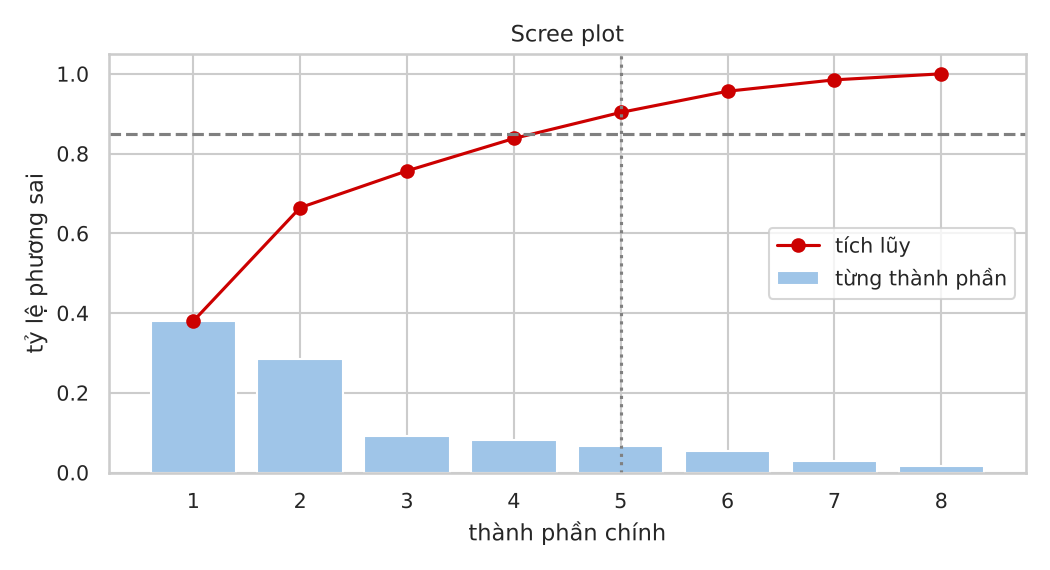
\includegraphics[width=\linewidth]{d_pca_variance.png}\end{minipage}\hfill
\begin{minipage}{0.56\linewidth}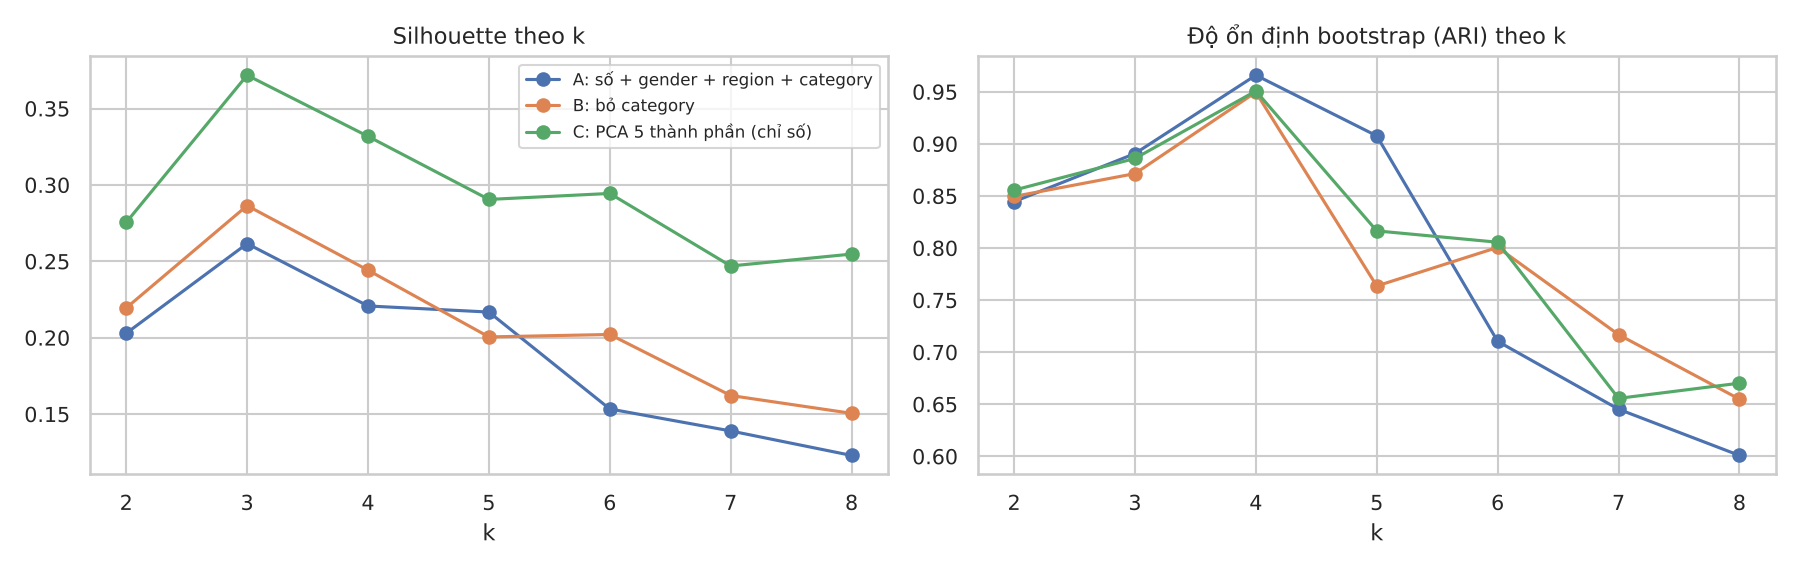
\includegraphics[width=\linewidth]{d_silhouette_k.png}\end{minipage}
\caption{Scree plot (trái); silhouette và độ ổn định bootstrap theo $k$ của ba phương án (phải).}
\end{figure}

\textbf{Chọn phương án} (silhouette trung bình $k = 3..6$, 3 mẫu bootstrap): A (số + gender + region + category, 17 cột) 0,213; B (bỏ category) 0,233; chỉ thuộc tính số 0,275; \textbf{C (PCA 5 thành phần) 0,322}. Độ ổn định của ba phương án tương đương (0,85--0,87). Chọn C. Các thuộc tính danh mục được loại khỏi không gian phân cụm và giữ lại để mô tả cụm.

\textbf{Không dùng Gower/K-Medoids:} K-Means cần không gian Euclid với tâm là trung bình; Gower chuẩn hóa theo khoảng [min, max] nên cực nhạy với ngoại lai (trên thang gốc 95\% khách nằm trong 5,7\% khoảng AOV); các thuộc tính danh mục ở đây lại không mang cấu trúc cụm. \textbf{Không giảm số đối tượng:} N = 220 đã nhỏ. \textbf{Không dùng \code{true\_segment}} ở bất kỳ bước nào. Kết quả: \code{customers\_prepared.csv}, \textbf{220 dòng $\times$ 6 cột} (\code{customer\_id} + PC1--PC5).

%=====================================================================
\section{Câu e. Phân cụm và đánh giá}

\textbf{Thiết lập.} K-Means (\code{n\_init = 10}, seed 2476). \emph{Trước xử lý}: dữ liệu bẩn với biến đổi tối thiểu để chạy được (điền median/mode, one-hot), 23 chiều trên thang gốc. \emph{Sau xử lý}: 5 thành phần chính. Cùng 220 khách, cùng \code{customer\_id}; \textbf{không gian đặc trưng khác nhau} nên silhouette và Davies--Bouldin không so sánh trực tiếp được. Chỉ số chính là \textbf{ARI, NMI} so với \code{true\_segment}; ngoài ra tính silhouette của cả hai bộ nhãn trên cùng một không gian tham chiếu (8 thuộc tính số đã log và chuẩn hóa). $k$ do silhouette chọn ($k = 2..8$), kèm kết quả $k = 4$.

\begin{table}[H]\centering\small
\begin{tabular}{@{}lcccc@{}}\toprule
 & \multicolumn{2}{c}{Trước xử lý} & \multicolumn{2}{c}{Sau xử lý}\\\cmidrule(lr){2-3}\cmidrule(lr){4-5}
 & $k = 2$ (chọn) & $k = 4$ & $k = 3$ (chọn) & $k = 4$\\\midrule
Kích thước cụm & 217, 3 & 183, 29, 5, 3 & 86, 74, 60 & 69, 63, 59, 29\\
ARI & 0,011 & 0,179 & \textbf{0,751} & \textbf{0,864}\\
NMI & 0,039 & 0,367 & 0,792 & 0,829\\
Silhouette (không gian riêng) & 0,978 & 0,692 & 0,372 & 0,332\\
Silhouette (không gian tham chiếu) & 0,494 & 0,181 & 0,327 & 0,286\\\bottomrule
\end{tabular}
\caption{So sánh hai kịch bản. ARI giữa hai bộ nhãn trước và sau: $-0{,}004$.}
\end{table}

\begin{figure}[H]\centering
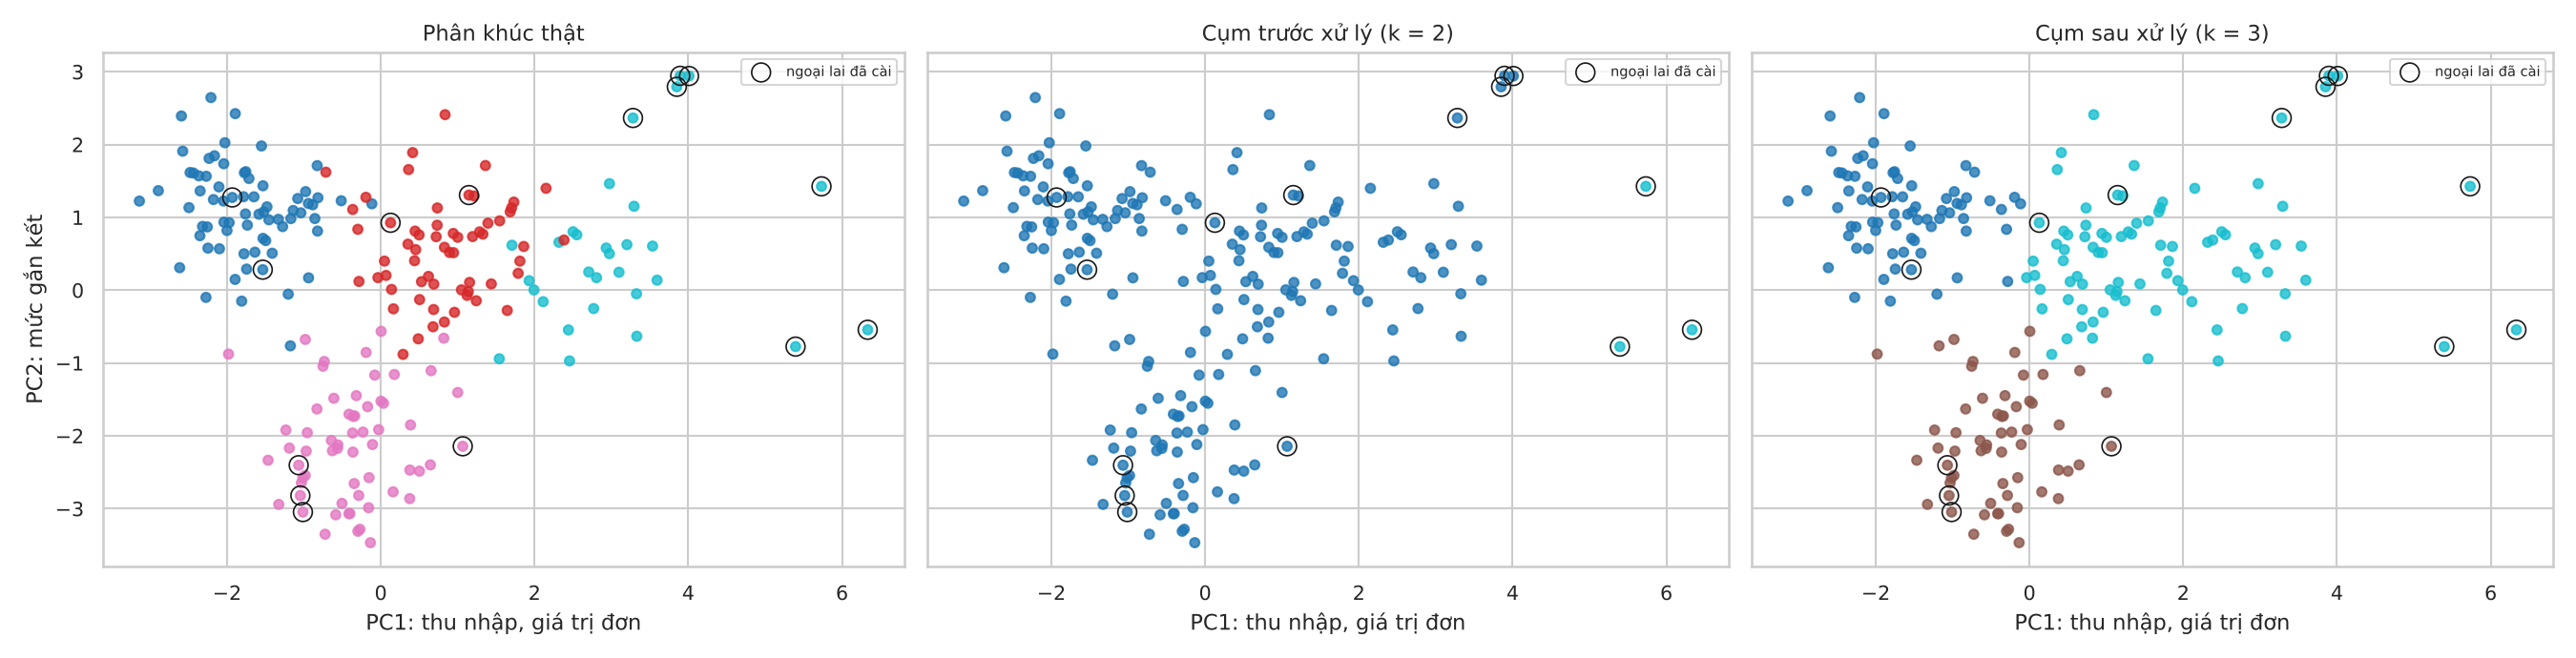
\includegraphics[width=\linewidth]{e_clusters_2d.png}
\caption{Phân khúc thật và các cụm, chiếu lên mặt phẳng PC1--PC2 (vòng tròn: ngoại lai đã cài).}
\end{figure}

\textbf{Phân tích sự thay đổi.} Trước xử lý, \code{avg\_order\_value} chiếm 98,2\% tổng phương sai; K-Means chỉ cô lập 3 khách siêu VIP (ARI 0,011, gần như ngẫu nhiên). Silhouette 0,978 là \emph{vô nghĩa}: cô lập vài điểm xa luôn cho silhouette cao. Sau xử lý, ARI tăng lên 0,751 ($k = 3$) và 0,864 ($k = 4$). 7 khách cực trị hợp lệ nằm trong cụm giá trị cao (ARI khi bỏ 7 dòng này: 0,776), xác nhận việc giữ chúng ở câu c không gây hại. Kết quả ổn định qua 20 seed (0,751 $\pm$ 0,000).

\textbf{Đặc điểm cụm sau xử lý} (median, thang gốc):
\begin{table}[H]\centering\small
\begin{tabular}{@{}p{3.3cm}cp{6.6cm}p{4.5cm}@{}}\toprule
Cụm & Quy mô & Đặc điểm & Hành động gợi ý\\\midrule
Săn khuyến mãi, mua thường xuyên & 74 (34\%) & 25 tuổi; 43 đơn/năm; giá trị đơn 231; khuyến mãi 72\%; hoàn 18\% & Voucher theo ngưỡng giỏ hàng; kiểm soát hoàn hàng\\
Mới hoặc ít hoạt động & 60 (27\%) & Gắn bó 3 tháng; 3 đơn/năm; 122 ngày chưa mua & Kích hoạt lại; ưu đãi đơn thứ hai\\
Trung thành, giá trị cao & 86 (39\%) & 39 tuổi; gắn bó 51 tháng; thu nhập 361; giá trị đơn 747 & Chăm sóc ưu tiên; bán chéo\\\bottomrule
\end{tabular}
\end{table}
Với $k = 4$, cụm thứ ba tách thành \emph{Trung thành tầm trung} (63) và \textbf{VIP} (29 khách, 13\%; thu nhập 664, giá trị đơn 2.013, Platinum, 59\% ưa Điện tử, khuyến mãi 19\%). gender ($p = 0{,}79$) và region ($p = 0{,}13$) không liên hệ với cụm; preferred\_category có liên hệ ($p < 0{,}001$) dù không dùng để phân cụm, hữu ích để mô tả và cá nhân hóa.

\textbf{Kiểm chứng các lựa chọn trước đó.} (i) \textbf{Silhouette chọn thiếu một cụm}: $k = 3$ gộp VIP với Trung thành; $k = 4$ đúng cấu trúc hơn (ARI 0,864). Khuyến nghị nghiệp vụ dùng 4 cụm. (ii) \textbf{PCA không giúp tìm đúng cấu trúc hơn}: ARI bằng bản không PCA ở $k = 3$ (0,751), hơi kém ở $k = 4$ (0,864 so với 0,885); mức tăng silhouette ở câu d là hiệu ứng của việc giảm số chiều. (iii) Thêm thuộc tính danh mục làm silhouette giảm nhưng ARI gần như không đổi (0,885 so với 0,889): loại chúng là vô hại chứ không cải thiện. \textbf{Tiêu chí thành công:} sau xử lý đạt cả 4; trước xử lý chỉ đạt silhouette, và đạt vì lý do sai.

%=====================================================================
\section{Kết luận, rà soát và hạn chế}
\textbf{Kết luận.} Tiền xử lý và chuẩn bị dữ liệu quyết định kết quả: ARI từ 0,011 lên 0,751 (0,179 lên 0,864 ở cùng $k = 4$). Nguyên nhân chính của thất bại trước xử lý là chênh lệch thang đo kết hợp cực trị, không phải giá trị thiếu hay nhiễu. Bài học về phương pháp: \textbf{silhouette không đáng tin trên dữ liệu này} (chọn sai $k$ trước xử lý, chọn thiếu cụm sau xử lý, phóng đại lợi ích của PCA).

\textbf{Rà soát nhất quán} (chạy lại toàn bộ pipeline): 5/5 notebook chạy không lỗi, dữ liệu tái lập giống hệt. Các điểm không nhất quán đã phát hiện và xử lý: (1) câu d ban đầu viết ``thuộc tính danh mục làm giảm chất lượng cụm''; câu e cho thấy điều này chỉ đúng theo silhouette, đã sửa lời nhận xét; (2) ở câu a, ``IQR không bắt được lỗi logic'' chỉ đúng khi xét các cột bị can thiệp; khi xét mọi cột (câu b) IQR thang gốc gắn cờ 2/3 dòng lỗi logic qua giá trị ở cột khác; (3) ngoại lai logic C0205 không phân biệt được với hành vi thật (lỗi thiết kế câu a); (4) hình và bảng của câu b, c nằm ở \code{reports/}, của câu d, e nằm ở \code{outputs/}.

\textbf{Hạn chế.} Dữ liệu giả lập có phân khúc tách biệt hơn thực tế nên ARI lạc quan; trong thực tế không có nhãn và phải dựa vào chỉ số nội tại vốn đã cho thấy kém tin cậy; chỉ thử K-Means; N = 220 nhỏ; người sinh dữ liệu đồng thời là người phân tích.

\textbf{Sản phẩm nộp} (Hình~\ref{fig:tree}): báo cáo; dữ liệu ban đầu và sau khi thêm nhiễu, ngoại lai (\code{data/raw}); dữ liệu sau tiền xử lý và chuẩn bị (\code{data/processed}); mã nguồn (\code{notebooks}, \code{src}); khai báo AI (\code{ai\_logs}).

\begin{figure}[H]\centering\footnotesize
\begin{forest}
for tree={font=\ttfamily\footnotesize, grow'=0, folder, s sep=0.6pt, l sep=6pt, inner ysep=0.6pt}
[{Midterm\_Data\_Mining/}
  [{README.md \quad\textrm{\itshape cấu trúc, cách chạy}}]
  [{requirements.txt}]
  [{data/}
    [{raw/ \quad\textrm{\itshape customers\_clean, customers\_dirty, injection\_log}}]
    [{processed/ \quad\textrm{\itshape preprocessed, prepared, scaled\_numeric, cluster\_assignments}}]]
  [{notebooks/ \quad\textrm{\itshape 01\_cau\_a … 05\_cau\_e (chạy tuần tự)}}]
  [{src/utils.py \quad\textrm{\itshape đường dẫn, lược đồ cột, ràng buộc, IQR}}]
  [{reports/}
    [{Bao\_Cao\_Ket\_Qua.tex / .pdf}]
    [{expected\_findings.md}]
    [{figures/, tables/ \quad\textrm{\itshape hình và bảng câu b, c}}]]
  [{outputs/}
    [{figures/, tables/ \quad\textrm{\itshape hình và bảng câu d, e}}]]
  [{ai\_logs/ \quad\textrm{\itshape AI\_DECLARATION.md, lịch sử hội thoại}}]
]
\end{forest}
\caption{Cấu trúc thư mục sản phẩm nộp.}\label{fig:tree}
\end{figure}

\textbf{Sử dụng AI.} Bài làm thực hiện cùng Claude (Anthropic); sinh viên phân tích đề, phản biện và quyết định các lựa chọn chính (giữ gender làm phép thử, nhiễu riêng cho recency, chất vấn rủi ro thiên kiến, chọn $k$ trong KNN, đặt NaN và gắn cờ cho ô bất khả). Chi tiết trong \code{ai\_logs/AI\_DECLARATION.md} và lịch sử hội thoại.

\end{document}
